\lab{Symbolic Computation in Python}{SymPy}
\label{lab:SymPy}

\objective{Become familiar with some of the basic tools available in SymPy}

Python is good for more than just analysis of numerical data.
There are several packages available which allow symbolic computation in Python.
One such package is SymPy.
SymPy is designed to be a fully featured computer algebra system in Python.
It is actually used for much of the symbolic computation in Sage.
An example of what we mean by "symbolic computation" is the following:
\begin{lstlisting}
import sympy as sy
x = sy.symbols('x')
sy.expand((x+1)**10)
\end{lstlisting}
which will return the following:
\begin{lstlisting}
x**10 + 10*x**9 + 45*x**8 + 120*x**7 + 210*x**6 + 252*x**5 + 210*x**4 + 120*x**3 + 45*x**2 + 10*x + 1
\end{lstlisting}
When used properly, this package can simplify large amounts of algebra for you.
This can be incredibly useful in a wide variety of situations.
As you may have guessed, such packages generally have a wide variety of features.
If you want to know how to do something, consider checking the documentation  at the SymPy website (\url{http://sympy.org/en/index.html}).
This lab should teach you to do some basic symbolic manipulations in SymPy, but keep in mind that this introduction is not comprehensive.

\section*{Some Convenient Tools}

Sympy includes a simplified plotting wrapper around Matplotlib.
A simple example is:
\begin{lstlisting}
x = sy.symbols('x')
expr = sy.sin(x)*sy.exp(x)
sy.plot(expr, (x, -3, 3))
\end{lstlisting}
which will plots $\sin\left(x\right) e^x$ for values of $x$ from -3 to 3.

SymPy also has several nice options for printing equations.
If you want to get a rough idea of what the equation looks like, you can use \li{sy.pprint()}.
It can interface with the IPython Notebook to display the formula more clearly as well.
If you are using the IPython Notebook, you can enable pretty printing by loading the extension that comes with SymPy.
In SymPy 7.2 this is done like this:
\begin{lstlisting}
%load_ext sympy.interactive.ipythonprinting
\end{lstlisting}
In SymPy 7.3 it is:
\begin{lstlisting}
import sympy as sy
sy.init_printing()
\end{lstlisting}
SymPy has many more useful features.
When in doubt, take a look at the SymPy documentation.
Figure \ref{sympy:pretty_printing} shows a screenshot of SymPy's special printing in the IPython notebook.
If at some point you need to write a formula in \LaTeX, the function \li{sy.latex()} can convert a SymPy symbolic expression to \LaTeX{} for you.

\begin{figure}
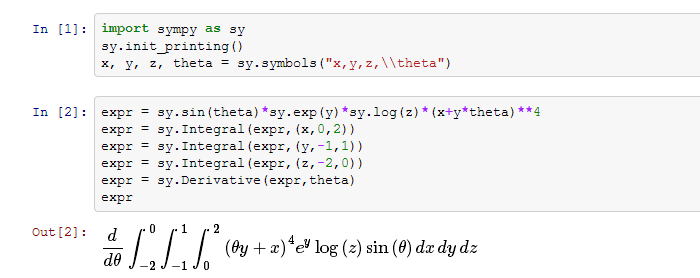
\includegraphics[width=\textwidth]{pretty_printing.png}
\caption{A screenshot showing how SymPy can interface with the IPython Notebook to display equations nicely.}
\label{sympy:pretty_printing}
\end{figure}

\section*{Basic Number Types}
SymPy has some good built in datatypes which can be used to represent rational numbers and arbitrary precision floating point numbers.
Arbitrary precision floating point operations are supported through the package \li{mpmath}.
These can be useful if you need to do computation to a very high precision, or to avoid possible overflow error in computation.
They are, however, much more costly to compute.

You can declare a rational number $\frac{a}{b}$ using \li{sy.Rational(a, b)}.
A real number $r$ of precision $n$ can be declared using $sy.Float(r,n)$.

A nice example of the use of these datatypes is the following function which computes $\pi$ to the $n$th digit.
\begin{lstlisting}
def mypi(n):
    #calculates pi to n decimal points.
    tot = sy.Rational(0, 1)
    term = 1
    bound = sy.Rational(1, 10)**(n+1)
    i = 0
    while bound <= term:
        term = 6 * sy.Rational(sy.factorial(2*i), 4**i*(sy.factorial(i))**2*(2*i+1)*2**(2*i+1))
        tot += term
        i += 1
    return sy.Float(tot, n)
\end{lstlisting}
This function works by evaluating the Taylor Series for $6\arcsin\left(\frac{1}{2}\right)$.
We used a rather crude error estimate to ensure that we were close enough to break the loop.

\begin{problem}
Write a function \li{myexp} that takes an integer $n$ as a parameter and evaluates $e$ to the $n$th digit, using an approach similar to the code given above.
Use the series 
\begin{equation*}
e=\sum_{n=0}^{\infty} \frac{1}{n!}
\end{equation*}
Use the same condition as above to determine when to break your while loop.
\end{problem}

\section*{Symbolic Manipulation}
In SymPy, you need to declare symbolic objects before you use them.
To define a symbol $x$, we write \li{x = sy.symbols('x')}.
This can also be used to define multiple variables at once, as in \li{x, y, z = sy.symbols('x,y,z')}.
The string form of each variable on the right is used for showing expressions that involve the variable.
You will need to be careful about capitalization and that last `s' in the name of the function.
Calling \li{sy.Symbol()} will allow you to create a single symbolic variable, but \li{sy.symbol} is a submodule and cannot be called at all.

SymPy can be used to solve difficult expressions for given variables.
Not everything can be solved, but SymPy's algorithms are pretty good and can often save a great deal of time.
We consider the following equation:
\begin{equation*}
\frac{w}{w-x}+\frac{x}{x-y}+\frac{y}{y-z}+\frac{z}{z-w}=0
\end{equation*}
Say we need an explicit solution for a given variable. 
Since the expression is symmetrical, it doesn't really matter which one, but we can solve this in the following way:
\begin{lstlisting}
import sympy as sy
w, x, y, z = sy.symbols('w, x, y, z')
expr = w/(w-x) + x/(x-y) + y/(y-z) + z/(z-w)
sy.solve(expr, w)
\end{lstlisting}
In any variable, this expression is quadratic, but each coefficient will depend on the other 3 variables.
This would be a terrible pain to do by hand, but SymPy can take care of that for us.
It is worth noting that SymPy cannot do everything, but if we keep in mind what we are doing and are familiar with the tools it has, it can make complex algebraic operations a great deal faster. 
We should also note that \li{solve()} returns a list of expressions.
If we want an expression to work with, we must take an item from the list.

In this particular example, you will notice that we only used a symbolic expression and not a full equation.
What SymPy did was set the expression equal to zero, solve for the variable we wanted, then return the result.
SymPy also supports equation objects (and inequalities), but this approach is often easier.
If you need to declare equations, they can be declared using something like \li{equation = Eq(x,  y)} which represents the equation $x=y$

\begin{problem}
Use SymPy to solve the equation $y=e^x+x$ for $x$.
The SymPy syntax for $e^x$ is simpy \li{sy.exp(x)}, provided that $x$ has been initialized as a symbol.
The answer will be in terms of the Lambert W function, which is a special function available in most major symbolic math libraries.
It is included in both SciPy and SymPy and is defined as the inverse of $y=x e^x$.
\end{problem}

SymPy can also be used to expand and simplify different symbolic expressions.
As an example we will simplify the expression
\begin{equation*}
\frac{w x^2 y^2 - w x^2 - w y^2 + w - x^2 y^2 z + 2 x^2 y^2 + x^2 z - 2 x^2 + y^2 z - 2 y^2 - z + 2}{w x y - w x - w y + w - x y z + 2 x y + x z - 2 x + y z - 2 y - z + 2}
\end{equation*}
\begin{lstlisting}
w, x, y, z=sy.symbols(`w, x, y, z')
expr = (w*x**2*y**2 - w*x**2 - w*y**2 + w - x**2*y**2*z + 2*x**2*y**2 + x**2*z - 2*x**2 + y**2*z - 2*y**2 - z + 2)/(w*x*y - w*x - w*y + w - x*y*z + 2*x*y + x*z - 2*x + y*z - 2*y - z + 2)
expr.simplify()
\end{lstlisting}
When we evaluate this cell, we can see that the expression simplifies to $x y + x + y +1$.
\li{simplify()} is the general simplification method for a SymPy expression.
It can be called as a function from the module, i.e. as \li{sy.simplify()} or it can be used as a method for an object as in the example above.
You can also tell SymPy to do more specific types of simplification, for example if you want to factor an expression, you can use \li{factor()}.
If you want to tell it to expand an expression you can use \li{expand()}, if you want it to focus purely on simplifying the trigonometric aspects of the expression you can use \li{trigsimp()}.
If you want SymPy to cancel variable expressions in the numerator and denominator of all rational sub-expressions, use \li{cancel()}.
There are several other kinds of algebraic manipulations you can do in SymPy, see the documentation for a more comprehensive list.
Many of these more important functions in SymPy are also available as methods to expressions.
This is the case with all of the above examples.

Be sure to be careful when writing out symbolic expressions.
Python floating point numbers are still floating point numbers and Python integers are still integers.
A simple example is the expression \li{(3/4)*sy.sin(x)} which evaluates to 0, and should probably have been written as \li{3*sy.sin(x)/4} or \li{sy.Rational(3,4)*sy.sin(x)}.
Be careful about using floating points as well.
The expression \li{(3./4.)*sy.sin(x)} will evaluate to \li{.75*sy.sin(x)}, and the floating point calculations will be carry through to the rest of your symbolic work with that expression.

Another useful feature is substitution.
Substitution can be done using the \li{subs()} method of an expression.
%As of this writing, there is no subs function, though one has been discussed.
%I deliberately left the ambiguity here for compatibility with future releases.
You can substitute numbers and variables in for variables and even expressions.
For example, if you want to see what an expression looks like if $x$ is set to zero, you can use:
\begin{lstlisting}
expr.subs(x, 0)
\end{lstlisting}
where \li{expr} is the expression you have already defined.
Note that none of these operations modify the expression in place.
They return a modified version of the expression, but do not actually change the original.

Substitution also can be used (to some extent) to substitute one expression for another .
For example, if you want to apply the double angle identity to replace products of sines and cosines, you could use the following:
\begin{lstlisting}
expr.subs(sy.sin(x) * sy.cos(x), sy.sin(2*x)/2)
\end{lstlisting}
If you want to eliminate higher powers of a variable in an expression you can use something like:
\begin{lstlisting}
expr.subs(x**3, 0)
\end{lstlisting}
which will eliminate all terms of the expression involving $x^3$.
At present time this will not eliminate terms involving $x^4$ or higher powers of $x$ that are not divisible by 3.

\begin{problem}
Problems of the following form are useful in proving that finite difference schemes remain bounded as the number of iterations increases.
This property is called stability and will be discussed later in Volume 4.
Here we will just walk you through the symbolic manipulations necessary to show that a scheme is stable.
Consider the Crank-Nicolson finite difference scheme for the partial differential equation $u_t+a u_x=0$.
\begin{equation*}
\frac{v_{m}^{n+1}-v_{m}^{n}}{k}+a\frac{v_{m+1}^{n+1}-v_{m-1}^{n+1}+v_{m+1}^{n}-v_{m-1}^{n}}{4h}=0
\end{equation*}
Due to an important result by Von Neumann, we know that this scheme will be stable if and only if when we make the following substitutions, the absolute value of the amplification factor $g$ is always less than or equal to 1.
Prove that this scheme is stable in the following way:
\begin{itemize}
\item Substitute $g^b e^{i c \theta}$ for $v_c^b$.
Note that when you have solved the expression for $g$, $g$ will be a function of $\theta$.
You are free to assume that $\theta$, $h$, and $k$ are real.
You can tell SymPy that these variables are real by including the argument \li{real=True} in the \li{symbols} function when you declare them.
$g$ may or may not be real, depending on the problem.
\li{sy.I} is the imaginary unit $i$.
\item Use SymPy to cancel redundant terms, simplify the expression, and solve for $g$.
Since the whole expression is set to zero, factor it, look at the factors and cancel all you can.
You will want to apply Euler's formula before you solve for $g$.
In this case we only want to make this particular substitution, so do this using the \li{subs()} method.
\item Once you have an expression for $g$, we may consider $\abs{g}^2$, which can be found by multiplying $g$ by the complex conjugate of $g$. 
You can take the conjugate of an expression using the \li{.conjugate()} method.
In this case, $\abs{g}$ should always be $1$, which shows that this scheme is stable for any $h$ and $k$.
\end{itemize}
\end{problem}

\section*{Calculus in SymPy}
SymPy can also be used to take limits, integrals, and derivatives.
Again, this can be very helpful when doing things that would be difficult to do by hand.
For example, the following equation takes the 20'th partial derivative with respect to $x$ of 
\begin{equation*}
\prod_{i=1}^{23} \left(x+i y\right)
\end{equation*}
\begin{lstlisting}
x, y, i = sy.symbols('x, y, i')
expr = sy.product((x+i*y), (i, 1, 23))
expr = expr.expand()
expr.diff(x, 20)
\end{lstlisting}

We can also integrate difficult things, for example, if we want to integrate $e^x\sin(x)\sinh(x)$, this can be done with one line in SymPy.
\begin{lstlisting}
sy.Integral(sy.sin(x) * sy.exp(x) * sy.sinh(x), x).doit()
\end{lstlisting}
Notice the \li{.doit()} method.
This tells SymPy to evaluate all derivatives, integrals, limits, etc. inside the expression.

Derivatives can be taken using the \li{sy.Derivative()} function, or the \li{.diff()} method of a SymPy expression.
As an example, we will take the 20'th derivative of the Lambert W function we saw earlier.
This can be done like this:
\begin{lstlisting}
from sympy.functions.elementary.exponential import LambertW
sy.Derivative(LambertW(x), x, 20).doit()
\end{lstlisting}
or, equivalently, like this:
\begin{lstlisting}
from sympy.functions.elementary.exponential import LambertW
LambertW(x).diff(x, 20).doit()
\end{lstlisting}
the second argument is the number of derivatives to take.
If it is omitted, one derivative will be taken.
You can also pass additional variables as arguments, for example, if we want to take $\frac{\partial}{\partial x} \left( \frac{\partial}{\partial y}\sin\left(x y\right)\right)$, we can do it in this way:
\begin{lstlisting}
expr = sy.sin(x*y)
expr.diff(x,y)
\end{lstlisting}
These tricks also work with integrals, with the exception of taking multiple integrals in the same variable.
You can integrate two different variables along two different bounds, as in:
\begin{lstlisting}
sy.integrate(y**2*x**2, (x, -1, 1), (y, -1, 1))
\end{lstlisting}
and you can integrate with respect to multiple variables, as in:
\begin{lstlisting}
sy.integrate(y**2 * x**2, x, y)
\end{lstlisting}
But, as of this writing, you can \emph{not} do something of the sort:
\begin{lstlisting}
sy.integrate(x**3, x, 20)
\end{lstlisting}
You would have to do this with some sort of for loop, or, simply by passing 20 $x$'s as arguments to the function.

SymPy also supports numerical integration and differentiation. 
If you want to evaluate a definite integral, something like this will work.
\begin{lstlisting}
sy.Integral(sy.sin(x)*sy.exp(x)*sy.sinh(x), (x, -1, 1)).doit()
\end{lstlisting}
This sort of thing will still return a purely symbolic expression, but you can get an actual value for it by either converting it to a SymPy \li{Float} object, or by using the \li{sy.N()} function, which numerically evaluates expressions as best as it can.
SymPy can also evaluate integrals numerically without finding a symbolic solution. That can be done like this:
\begin{lstlisting}
sy.N(sy.Integral(sy.sin(x)*sy.exp(x)*sy.sinh(x), (x, -1, 1)))
\end{lstlisting}
If for some reason you wanted to evaluate the expression to more digits of precision, you can add the number of significant digits as an argument to \li{sy.N()}.

\begin{problem}
Use SymPy to symbolically evaluate 
\begin{equation*}
\int_0^\infty \sin\left(x^2\right) dx
\end{equation*}
In SymPy, positive infinity is represented by the object \li{sy.oo}
\end{problem}

\begin{problem}
Use SymPy to numerically estimate $\frac{\partial}{\partial x}e^{\sin\left(\cos\left(x\right)\right)}$ at $x=1$.
\end{problem}

You can also use SymPy to solve some sorts of basic ordinary differential equations.
This will solve the equation $y_{xx}-2*y_x+y=\sin\left(x\right)$
\begin{lstlisting}
x = sy.symbols('x')
f = sy.Function('f')
eq = sy.Eq(f(x).diff(x, 2) - 2*f(x).diff(x) + f(x), sy.sin(x))
sy.dsolve(eq)
\end{lstlisting}
or, equivalently,
\begin{lstlisting}
x = sy.symbols('x')
f = sy.Function('f')
expr = f(x).diff(x, 2) - 2*f(x).diff(x) + f(x) - sy.sin(x)
sy.dsolve(expr)
\end{lstlisting}
\begin{problem}
Use SymPy to solve the following differential equation:
\begin{equation*}
\begin{split}
 y_{xxxxxx} & + 3y_{xxxx} + 3y_{xx} + y = \\
& x^{10}e^x + x^{11}\sin\left(x\right) + x^{12}e^x\sin\left(x\right) -x^{13}\cos\left(2x\right) + x^{14}e^x\cos\left(3x\right)
\end{split}
\end{equation*}
You may recall from your last class on differential equations that this sort of problem is solved by the method of undetermined coefficients. 
Imagine how terrible this would be to do by hand!
\end{problem}

In addition, SymPy includes several integral transforms, such as the Laplace, Fourier, Sine, and Cosine Transforms.
SymPy also allows you to do simple separation of variables on PDEs, Taylor Series, Laurent Series, Fourier Series, and many, \textit{many} other things.

\section*{Interfacing With Numerical Software}
SymPy also has a variety of built in ways to take an expression and turn it into a python function that can be evaluated quickly.
You can numerically evaluate expressions using \li{subs} to substitute in values like you would symbols, but this can be slow for large arrays.
A simple way to evaluate an expression more quickly is the \li{lambdify} function in \li{sympy.utilities.lambdify}.
It takes an expression and makes it into a callable python function. 
It allows you to specify which library to use to compute the function, so if you would like to operate on arrays, you can use NumPy functions for $\sin$, $\cos$, etc.
It also allows you to tell it to use functions from the math library, SymPy itself, and mpmath.
We can take an expression in $x$ and $y$ and make a corresponding python function \li{fc} which uses NumPy as its backend in the following way:
\begin{lstlisting}
import sympy as sy
from sympy.utilities.lambdify import lambdify
import numpy as np
x, y = sy.symbols('x, y')
expr = sy.sin(x) * sy.exp(x) - sy.cosh(x)
fc = lambdify([x, y], expr, 'numpy')
\end{lstlisting}
This interoperability allows us to move quickly between symbolic calculations in SymPy and faster numerical evaluation on arrays in NumPy.

SymPy also has built in ways that allow you to make functions that iterate over arrays using F2PY, Cython, or Theano.
Using these other libraries can result in very fast numerical evaluation of symbolic expressions with relatively little effort.
These automatic wrapping features depend on other libraries and may require some setup.

\begin{problem}
Use the \li{lambdify} function to make a NumPy-dependent function for your solution to the previous problem.
Set all the constants that would come from the initial conditions equal to 1.
The solution to the differential equation is an equality, but you can get the right hand side of the equality using \li{expr.rhs}.
Use the function you have just defined to plot the solution from -3 to 3.
It should be very large, and should look kind of like a sine curve.
\end{problem}
